\documentclass{article}


 % Required for inserting code snippets
\usepackage{mathtools}
\usepackage{graphicx}
\usepackage{subfig}
\usepackage{verbatim}
\usepackage{algpseudocode}
\usepackage{natbib}
\usepackage{url}
\usepackage{listings}
\usepackage{float}
\usepackage{array}
\usepackage{booktabs}
\usepackage{amssymb}
%\setcounter{MaxMatrixCols}{16}

%%%%%%%%%%%%%%%%%%%%%%%% PAINTING LIBRARY
\usepackage{pgf}
\usepackage{tikz}
\usetikzlibrary{arrows,automata}
\usepackage[latin1]{inputenc}
\usepackage[upright]{fourier}
\usetikzlibrary{matrix}
\usepackage{fullpage,amsmath}
\usepackage{times}
\usepackage{geometry}
\usetikzlibrary{mindmap,backgrounds}

%%%%%%%%%%%%%%%%%%%%%%%% THNX TO OZAN FOR THE CODE HEADER ;)
\usepackage{color}
\usepackage{xcolor}
\usepackage{listings}

\usepackage{courier}
\definecolor{DarkGray}{rgb}{0.43,0.35,0.35} % Comment color
\lstset{
	language=C++,								% choose the language of the code
		basicstyle=\footnotesize\ttfamily,  % the size of the fonts that are used for the code
		numbers= left,						% where to put the line-numbers
		numberstyle=\tiny,					% the size of the fonts that are used for the line-numbers
		stepnumber=1,						% the step between two line-numbers. If it is 1 each line will be numbered
		numbersep=10pt,						% how far the line-numbers are from the code
		backgroundcolor=\color{white},		% choose the background color. You must add \usepackage{color}
		keywordstyle=\color{DarkGray}\bf,
	showspaces=false,						% show spaces adding particular underscores
		showstringspaces=false,				% underline spaces within strings
		showtabs=false,						% show tabs within strings adding particular underscores
		keywordstyle=\color{DarkGray}\bf,
		stringstyle=\color[rgb]{0.627,0.126,0.941},
		xleftmargin=17pt,
		framexleftmargin=17pt,
		framexrightmargin=5pt,
		framexbottommargin=4pt,
		%frame=b,         
		frame=single,					% adds a frame around the code
		tabsize=2,						% sets default tabsize to 2 spaces
		captionpos=t,					% sets the caption-position to bottom (t=top, b=bottom)
		breaklines=true,				% sets automatic line breaking
		breakatwhitespace=false,		% sets if automatic breaks should only happen at whitespace
		escapeinside={\%*}{*)}          % if you want to add a comment within your code
}

\usepackage{caption}
\DeclareCaptionFont{white}{\color{white}}
\DeclareCaptionFormat{listing}
{
	\colorbox[rgb]{0.83, 0.85, 0.88}
	{\parbox{\dimexpr\textwidth-8\fboxsep\relax}{#1#2#3}}
}

\captionsetup[lstlisting]
{
	format=listing,
		labelfont=white,
		textfont=white, 
		singlelinecheck=false, 
		margin=0pt, 
		font={bf,footnotesize}
}

\usepackage{textcomp}

%%%%%%%%%%%%% WATERMARKS  %%%%%%%%%%%%%%%%%
%\usepackage{eso-pic}
%\AddToShipoutPicture{
%    \includegraphics[width=1.74\textwidth,natwidth=1223,natheight=121]{figs/lowImg2.png}}

\DeclarePairedDelimiter\abs{\lvert}{\rvert}


%%%%%%%%%%%%% PARAGRAPHS %%%%%%%%%%%%%%%%%
%No ident in new paragraph
\usepackage[parfill]{parskip}
%% Add a space of 1.5 lines between paragraphs
\parskip=1.1\baselineskip

%%%%%%%%%%%%% DEFAULT FONT %%%%%%%%%%%%%%%
%Sans-serif font by default
%\renewcommand{\familydefault}{\sfdefault}
%\usepackage{mathptmx}

%\usepackage{bookman}
%%%%\usepackage[default]{droidserif}
%\usepackage[T1]{fontenc}
%\usepackage{lxfonts}
%\usepackage{tgadventor}
%\renewcommand*\familydefault{\sfdefault} %% Only if the base font of the document is to be sans serif
%\usepackage[T1]{fontenc}


\newcommand{\specialcell}[2][c]{%
  \begin{tabular}[#1]{@{}c@{}}#2\end{tabular}}

\usepackage{float}


\begin{document}
\title{Report Homework 3}
\date {\today}
\author{Tatiana Lopez Guevara}
\maketitle

\section{Problem 1}

In the problem we have 2 different groups of people: those who read the paper on Day n $(g_1)$ 
and those who don't buy it $(g_2)$. 
Therefore, as the suggestion says, we can define the following
vector:

\begin{equation*}
\begin{aligned}
v_n = 
\left(
\begin{array}{c}
g_1\\ 
g_2
 \end{array}
 \right)
 \in
 \mathbb{R}^2
\end{aligned}
\end{equation*} 

where $g_1$ is the size of the group 1 and $g_2$ is the size of the group 2.

Since we are dealing with Markov Processes, we know that we are modeling the
movement of people from one group to another with no gain or loss. This means,
 the total population is always conserved.

\subsection{Question 1}

If we belong to $g_1$ then, on the next day, we will have two possibilities:
not purchasing the newspaper or purchasing and reading it. 
The problem tells us that the probability of reading the newspaper on the next day
if we already purchased it its 0.7, which also means that the other option 
(move to $g_2$) will happen with a probability of 0.3.
By performing the same analysis for the second group $(g_2)$ we obtain the 
following Markov state graph:

\begin{figure}[H]
\begin{center}
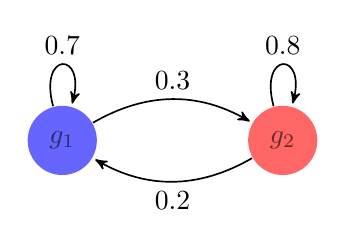
\begin{tikzpicture}[->,>=stealth',shorten >=1pt,auto,node distance=2.8cm,semithick]
\tikzstyle{every state}=[fill=blue,draw=none,text=black,opacity=.6]
\node[state]		 (A)             {$g_1$};
\tikzstyle{every state}=[fill=red,draw=none,text=black,opacity=.6]
\node[state]         (B) [right of=A] {$g_2$};

\path 
(A) edge [loop above] node        {$0.7$} (A) 
    edge [bend left ] node[above] {$0.3$} (B)
(B) edge [loop above] node        {$0.8$} (B)
	edge [bend left ] node[below] {$0.2$} (A);
\end{tikzpicture}
\end{center}
\caption{State Transitions}
\label{fig:mg}
\end{figure}

Which in terms of a Markov matrix $M=(m_{ij})$ becomes figure \ref{fig:mm1}. 

\newcommand{\myunit}{1 cm}
\begin{figure}
\begin{center}
\tikzset{node style ge/.style={circle}}
\begin{tikzpicture}
% les matrices
\tikzset{BarreStyle/.style =   {opacity=.6,line width=7mm,line cap=round,color=#1}}
\matrix (M)  [	matrix of math nodes, 
				nodes = {node style ge},,
				column sep=0 mm,
				left delimiter  = (,%
				right delimiter = )] at (0,0)
{ 0,7 & 0.2 \\
  0.3 & 0.8 \\
};

\draw [BarreStyle=blue] (M-1-1.north) to (M-2-1.south);
\draw [BarreStyle=red](M-1-2.north) to (M-2-2.south);
\matrix (M1)  [	matrix of math nodes, 
				nodes = {node style ge},,
				column sep=0 mm,
				left delimiter  = (,%
				right delimiter = )] at (6*\myunit,0)
{ 0,7 & 0.2 \\
  0.3 & 0.8 \\
};
\draw [BarreStyle=blue] (M1-1-1.west) to (M1-1-2.east);
\draw [BarreStyle=red](M1-2-1.west) to (M1-2-2.east);
\end{tikzpicture}
\end{center}
\caption{Markov matrix M}
\label{fig:mm1}
\end{figure}

As we can see, each column $j$ contains all the possible transitions starting
from the state $g_j$ and therefore, since the system is conservative,
it must add up to 1 (figure \ref{fig:mm1} left). 
Moreover, each row $i$ is the probability to arrive at the state $i$ 
from any other state (figure \ref{fig:mm1} rigth).

\subsection{Question 2}

The matrix M represents which part of the population moves from one state to
another or the probability of a single person moving on the next day. 
This means, the probability to get to state in the day $k+1$ depends on
the incoming links to that state from the dat $k$.

\begin{equation}
\begin{aligned}
(g_1)_{n+1} = 0.7*(g_1)_n + 0.2*(g_2)_n \\
(g_2)_{n+1} = 0.3*(g_1)_n + 0.8*(g_2)_n
\end{aligned}
\end{equation} 

This can be expressed in a matricial form

\begin{equation}
\begin{aligned}
\left(
\begin{array}{c}
g_1\\ 
g_2
\end{array}
\right)_{n+1} 
&=
\begin{pmatrix}
 0,7 & 0.2\\
 0.3 & 0.8
 \end{pmatrix}
\left(
\begin{array}{c}
g_1\\ 
g_2
\end{array}
\right)_n \\
v_{n+1} &= M v_n
\label{eq:mm1}
\end{aligned}
\end{equation} 

\subsection{Question 3}

As stated before, we are dealing with a $v_{n+1} = Mv_n$ 
type of problem for which we already know the solution
can be expressed as:

\begin{equation*}
\begin{aligned}
v_{k+1} &= M^n v_0 \\
v_{k+1} &= S \Lambda^n S^{-1} v_0
\end{aligned}
\end{equation*} 

We can see that the powers of the matrix $M$ can be calculated using the 
diagonalized matrix $\Lambda$ and the eigenvector matrix $S$.
Since this is a Markov matrix we already know that there will be an eigenvalue
$\lambda_1$ = 1. To get the other eigenvalue we use the following nice property:

\begin{equation*}
\begin{aligned}
tr(M) = \lambda_1 + \lambda_2 = 0.15\\ 
\lambda_2 = 0.5
\end{aligned}
\end{equation*} 

Now, we get the eigenvectors for $\lambda_1$:

\begin{equation}
\begin{aligned}
\begin{pmatrix}
 -0.3 & 0.2\\
 0.3 & -0.2
 \end{pmatrix}
x_1
&=
\left(
\begin{array}{c}
0\\ 
0
 \end{array}
 \right) \\
x_1 &= 
\left(
\begin{array}{c}
2\\ 
3 
 \end{array}
 \right) 
\label{eq:mm1}
\end{aligned}
\end{equation} 

And the eigenvectors for $\lambda_2$:

\begin{equation}
\begin{aligned}
\begin{pmatrix}
 0.2 & 0.2\\
 0.3 & 0.3
 \end{pmatrix}
x_2
&=
\left(
\begin{array}{c}
0\\ 
0
 \end{array}
 \right) \\
x_2 &= 
\left(
\begin{array}{c}
-1\\ 
1 
 \end{array}
 \right) 
\label{eq:mm1}
\end{aligned}
\end{equation} 

Packing up everything, we have:
\begin{equation*}
\begin{aligned}
\Lambda &=
\begin{pmatrix}
1 & 0 \\
0 & 0.5
 \end{pmatrix}  \\
S &=
\begin{pmatrix}
2 & -1 \\
3 & 1
 \end{pmatrix} \\
 S^{-1} &= 
\begin{pmatrix}
 \frac{1}{5} & \frac{1}{5}\\ 
-\frac{3}{5} & \frac{2}{5}
\end{pmatrix} 
\end{aligned}
\end{equation*} 

\begin{itemize}
\item How likely is to purchase on Day 2? Day 3? Day n?
\end{itemize} 

On the Day n we see that the likelihood of moving from one state to
another is given by the $n_{th}$ power of the matrix $M$.

\begin{equation}
\begin{aligned}
v_2 &= M^2 v_0 \\
v_3 &= M^3 v_0 \\
v_n &= M^n v_0 \\
    &=S\Lambda^n S^{-1} v_0 \\
\end{aligned}
\label{eq:vn}
\end{equation} 

The probability to be in the group $g_1$ on Day n given that today (Day 0)
we bought it is the first position of $v_n$ and implies an initial state:

\begin{equation*}
\begin{aligned}
v_0 = 
\left(
\begin{array}{c}
1\\ 
0 
 \end{array}
 \right) 
\end{aligned}
\end{equation*} 

We will apply the equation (\ref{eq:vn}):

\begin{equation}
\begin{aligned}
v_2 &= M^2 v_0 \\ 
	&=(S\Lambda^2 S^{-1}) v_0\\
	     &=  
	S
	\begin{pmatrix}
	1 & 0 \\ 
	0 & 0.25
	\end{pmatrix}
	S^{-1} 
	\left(
	\begin{array}{c}
	1 \\ 
	0 
	 \end{array}
	 \right) \\
	  &=
	  \left(
	  \begin{array}{c}
	  0.55\\ 
	  0.45 
	   \end{array}
	   \right) 
\end{aligned}
\end{equation}

Which means there is a $55\%$ of probability that the person buys the paper on Day 2.

For the thrid day we have:

\begin{equation}
\begin{aligned}
v_3 &= M^3 v_0 \\ 
	&=(S\Lambda^3 S^{-1}) v_0\\
	     &=  
	S
	\begin{pmatrix}
	1 & 0 \\ 
	0 & 0.125
	\end{pmatrix}
	S^{-1} 
	\left(
	\begin{array}{c}
	1 \\ 
	0 
	 \end{array}
	 \right) \\
	  &=
	  \left(
	  \begin{array}{c}
	  0.475\\ 
	  0.525 
	   \end{array}
	   \right) 
\end{aligned}
\end{equation}

Which means there is a $47.5\%$ of probability that the person buys the paper on Day 3.

\begin{equation}
\begin{aligned}
v_n &= (S\Lambda^n S^{-1}) 
	\left(
	\begin{array}{c}
	1  \\
	0 
	 \end{array}
	 \right) \\
\end{aligned}
\end{equation}

When $n$ is suficiently large, we get to the stability condition where
$40\%$ of the people read the paper.

\begin{itemize}

\item What sales figures can \textit{The Computer Visionist} expect
on Day 2? Day 3? Day n?
\end{itemize} 

Since we want to know the sales figure,
we take into account all the population for the initial state.
\begin{equation*}
\begin{aligned}
v_0 = \left(
\begin{array}{c}
750\\ 
250 
 \end{array}
 \right) 
\end{aligned}
\end{equation*} 

So we only need to apply again (\ref{eq:vn}) 

\begin{equation}
\begin{aligned}
v_2 &= M^2 v_0 \\ 
	&=(S\Lambda^2 S^{-1}) v_0\\
	     &=  
	S
	\begin{pmatrix}
	1 & 0 \\ 
	0 & 0.25
	\end{pmatrix}
	S^{-1} 
	\left(
	\begin{array}{c}
	750 \\ 
	250 
	 \end{array}
	 \right) \\
	  &=
	  \left(
	  \begin{array}{c}
	  487.5\\ 
	  512.5 
	   \end{array}
	   \right) 
\end{aligned}
\end{equation}

This means that we expect around 488 people to buy the paper on the second day.

\begin{equation}
\begin{aligned}
v_3 &= M^3 \\
	&=(S\Lambda^3 S^{-1}) v_0\\
	     &=  
	S
	\begin{pmatrix}
	1 & 0 \\ 
	0 & 0.125
	\end{pmatrix}
	S^{-1} 
	\left(
	\begin{array}{c}
	750  \\
	250 
	 \end{array}
	 \right) \\
	  &=
	  \left(
	  \begin{array}{c}
	  443.75\\ 
	  556.25
	   \end{array}
	   \right) 
\end{aligned}
\end{equation}

Which means we expect around 444 people to buy the paper on Day 3.

\begin{equation}
\begin{aligned}
v_n &= (S\Lambda^n S^{-1}) 
	\left(
	\begin{array}{c}
	750  \\
	250 
	 \end{array}
	 \right) \\
\end{aligned}
\end{equation}

This is the expression for a given day $n$. However if $n$ is very large $(n\to\infty)$
then we get to the stability condition described in the following section.

\begin{itemize}
\item Will the sales figure fluctuate a great deal from day to day, or are they likely to
become stable eventually?
\end{itemize} 

We want to know the stability of the system. Therefore we must analyse what will
happen with $M$ in the Day $n\to\infty$.

As we could see in the last equation of (\ref{eq:vn}), if we take $n\to\infty$
the only value that will prevail in $\Lambda$ will be the eigenvalue 1.
The other value is less than one so after every power it will become lower and lower
and eventually will turn out to be 0.


\begin{equation}
\begin{aligned}
M^\infty &= 
	S 
	\begin{pmatrix}
	1 & 0 \\ 
	0 & 0.5 
	\end{pmatrix}^\infty
	S^{-1} \\
    &= \frac{1}{5} 
	\begin{pmatrix}
	2 & 2 \\ 
	3 & 3
	\end{pmatrix} \\
	&= \frac{1}{5} [x_1 x_1]
\end{aligned}
\end{equation} 

As expected, we obtain a matrix with the 
corresponding eigenvector of the eigenvalue = 1
and this is called the steady state.

\begin{equation*}
\begin{aligned}
v_\infty &=  M^\infty v_0\\
	     &=  \frac{1}{5} 
	\begin{pmatrix}
	2 & 2 \\ 
	3 & 3
	\end{pmatrix}
	\left(
	\begin{array}{c}
	750 \\ 
	250 
	 \end{array}
	 \right)
	  &=
	  \left(
	  \begin{array}{c}
	  400\\ 
	  600 
	   \end{array}
	   \right) 
\end{aligned}
\end{equation*} 

So the sales figure \textbf{will} become stable and the expected number of people
that will read the newspaper is 400.

\section{Google Page Rank}

The google page rank algorithm is a nice and powerful application of linear algebra. 
The stated problem was how to display the obtained results in a given order such that
the most important results relative to the user are shown first. 
The relevance of a website is given by its connection with other websites. 

In the first section of \cite{prank1} a very simple strategy is used: just create
and adjacency matrix $A_{NxN}$, whose entries describe the connection between $N$
different websites.
This means, if the cell $a_{ij} = 1$ then there is a link from the website $j$ to the
website $i$ and 0 means there is not. The value of a page $i$ is then defined as the sum
of all the references it has, which means a sum of the entries of the $row_i(A)$. This, 
expressed in a matricial form becomes:

\begin{equation*}
\begin{aligned}
v_i = P u \;,\; u \in \mathbb{R}^{N} 
\end{aligned}
\end{equation*} 

Where $u$ is an unitary vector.

The second improvement is to transform the matrix $A$ into a Markov matrix
$P$ by dividing each column with its sum. This step is performed in order to 
assign a relevance to each recommender which is inversely proportional
to the number of links it has. So, if one page has a lot of outgoing links,
then it is less important than one that has only a few.
Also, to avoid a division by zero, the dead ends 
are assumed to have the lowest possible value because they are modified to
have a reference to all web sites.

After that, a weight is given to each recommendation, and this means that
the matrix is multiplied by $v$ since this vector, as they describe, is the
value of each page.

\begin{equation*}
\begin{aligned}
v = P v
\end{aligned}
\end{equation*} 

By definition, the previous formula is stating that exists an eigenvalue = 1.
Of course, since $P$ is a Markov matrix!.

\subsection{Eigenvalue Problem}

The eigenvalue problem described occurs when we get more than one eigenvalue = 1.
This is due to clustering and thus the previous formula will not have a unique solution.
Also, since they are dealing with the entire web, there will be a lot of zero entries.
Here they apply a very nice trick to get a new Markov matrix whose entries are 
all >= 0 which is guaranteed to have the following properties 
for the eigenvector $v$ corresponding to
the $\lambda=1$:

\begin{itemize}
\item All entries of $v$ are positive
\item The sum of $v$ add up to 1
\item There exists an unique eigenvector for the $\lambda=1$
\end{itemize} 

The performed trick is just to add a "jumping" factor to a random
page called $r$. This value is usually set up to 0.85 for Google. 

This means that with an $r$ percent of probability the user will use the links
between the pages, but he can also jump (with an $1-r$ percent of probability) 
to go to a random site modeled by a Matrix $T$ whose entries all have the same
probability to be chosen.

\begin{equation}
\begin{aligned}
T = ones(N,N) / N	\\
Q = rP + (1-r)T
\end{aligned}
\label{eq:q}
\end{equation} 

A final nice trick is performed to calculate this eigenvector, that is to say,
the rank of the webpages which is related to another cool property of the matrix $Q$:

\begin{itemize}
\item Given any vector $w$ whose entries are positive and add up to 1, then $Q^k w$ 
converges to $v$ when $k\to\infty$.
\end{itemize} 

This is because, as we saw in the first section, 
when k is sufficiently large, we reach the stability condition no matter what is
the initial condition the result will converge to the eigenvector of $\lambda_1$

This allows to avoid the high complexity calculation of the eigenvector by
the traditional method, and instead use a numerical iterative method to approximate the
vector $v$. The only thing needed is an initial random vector $w$ that has such property, 
and sequentialy calculate $Q^k w$ until we find two results that are very similar, which means
it has converged. 

\begin{equation*}
\begin{aligned}
Q w &= r P w + (1-r) T w \\
	&= r P w + \frac{1-r}{N} u 
\end{aligned}
\end{equation*} 

Some other simplifications were made: $T w$ is the average of entries of $w$ so it is replaced by a vector
of ones divided by $N$.
This new term does not depend on $w$ which means the calculation
can be performed only once (before the iterations).
The $P w$ term is really
fast to calculate because $P$ is a sparse matrix, 
which means it has a lot of zeros.

\subsection{Example}

A matlab code implementation is attached to this report. It takes the adjacency matrix
$A$ (any size) and calculates the matrix $P$, $Q$ and the vector $v$. It also checks 
the given approximation of $v$ by actually obtaining the eigenvector of $\lambda_1$
with the traditional method. Finally, it shows a graph with each page represented
by a circle of a size proportional to the relevance it has.

The following matrix was used as the requested 5x5 example:
\begin{equation*}
\begin{aligned}
A=
\begin{pmatrix}
0&0&1&0&0\\
1&0&0&0&0\\
0&0&0&0&0\\
1&1&1&0&1\\
0&0&0&1&0
 \end{pmatrix} 
\end{aligned}
\end{equation*} 

Which is represented by the following graph:

\begin{center}
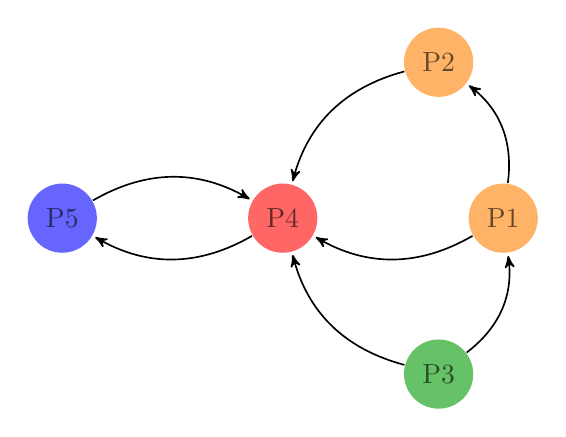
\begin{tikzpicture}[->,>=stealth',shorten >=1pt,auto,node distance=2.8cm,semithick]
\centering
\tikzstyle{every state}=[fill=blue,draw=none,text=black,opacity=.6]
\node[state]		 (P5)             {P5};
\tikzstyle{every state}=[fill=red,draw=none,text=black,opacity=.6]
\node[state]         (P4) [right of=P5] {P4};
\tikzstyle{every state}=[fill=green!60!black,draw=none,text=black,opacity=.6]
\node[state]         (P3) [below right of=P4] {P3};
\tikzstyle{every state}=[fill=orange,draw=none,text=black,opacity=.6]
\node[state]         (P2) [above right of=P4] {P2};
\tikzstyle{every state}=[fill=orange,draw=none,text=black,opacity=.6]
\node[state]         (P1) [right of=P4] {P1};

\path 
(P5) edge [bend left] node[above] {} (P4) 
(P4) edge [bend left] node[below] {} (P5)
(P3) edge [bend left] node[above] {} (P4)
     edge [bend right] node[above] {} (P1)
(P2) edge [bend right] node[above] {} (P4)
(P1) edge [bend left] node[above] {} (P4)
	 edge [bend right] node[below] {} (P2)
;
\end{tikzpicture}
\end{center}

By performing the RankPage algorithm we expect to find that the
relevance of the 4th page is greater than all the others and 
that since the 5th page is referenced by page 4th, then it
must also be very relevant. The expected results are shown in the 
following figure:

\begin{center}
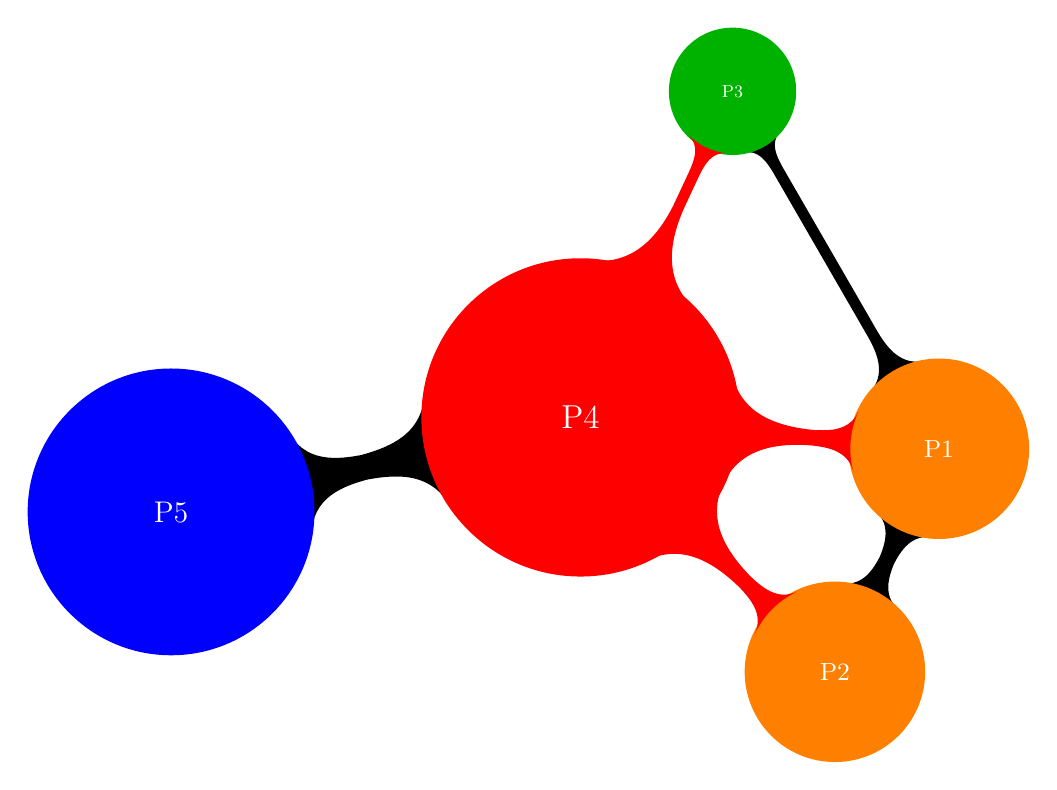
\begin{tikzpicture}[mindmap,
	level 1 concept/.append style={level distance=130,sibling angle=40}]
\centering
\begin{scope}[mindmap, concept color=red, text=white]
\node [concept] (P4) {P4}[clockwise from=-5] 
child {node [concept,color=orange,text=white] (P1) {P1}}
child {node [concept,color=orange,text=white] (P2) {P2}}
child [grow=65]{node [concept,scale=0.7,color=green!70!black,text=white] (P3) {P3}};
\end{scope}

\begin{scope}[mindmap, concept color=blue, text=white]
\node [concept, scale=0.9] (P5) at (-5.2,-1.2) {P5};
\end{scope}

\begin{pgfonlayer}{background}
\path (P1) to[circle connection bar, color=blue] (P2);
\path (P3) to[circle connection bar] (P1);
\path (P4) to[circle connection bar] (P5);
\end{pgfonlayer}
\end{tikzpicture}
\end{center}

The obtained results after running the code are:

\begin{equation*}
\begin{aligned}
P = 
\begin{pmatrix}
0&0&0.5000&0&0\\
0.5000&0&0&0&0\\
0&0&0&0&0\\
0.5000&1.0000&0.5000&0&1.0000\\
0&0&0&1.0000&0\\
\end{pmatrix} 
\end{aligned}
\end{equation*} 

\begin{equation*}
\begin{aligned}
Q &= 
\begin{pmatrix}
0.0300&0.0300&0.4550&0.0300&0.0300\\
0.4550&0.0300&0.0300&0.0300&0.0300\\
0.0300&0.0300&0.0300&0.0300&0.0300\\
0.4550&0.8800&0.4550&0.0300&0.8800\\
0.0300&0.0300&0.0300&0.8800&0.0300\\
\end{pmatrix} 
\end{aligned}
\end{equation*} 

\begin{equation*}
\begin{aligned}
w_{approx} = 
\left(
\begin{array}{c}
0.0428\\
0.0482\\
0.0300\\
0.4589\\
0.4201\\
 \end{array}
 \right) 
\end{aligned}
\end{equation*} 

\begin{equation*}
\begin{aligned}
v_{real} = 
\left(
\begin{array}{c}
0.0427\\
0.0482\\
0.0300\\
0.4590\\
0.4201\\
 \end{array}
 \right) 
\end{aligned}
\end{equation*} 

We can observe that the two obtained vectors 
(the approximated
through the iteration $w_{approx}$, 
and the real eigenvector $v_{real}$) are very similar.
The $\epsilon$ factor used as a stop condition was $10^{-4}$,
that is to say, the algorithm stops until the sum of the individual
errors between two consecutive obtained vectors is less or equal
than $\epsilon$.

\begin{figure}[h!]
\centering
\includegraphics[width=0.7\textwidth,natwidth=560,natheight=419]{result.png}
\caption{Plotted ranking of Pages ordered from 1 to 5 (left to right)}
\label{fig:rank}
\end{figure} 

\bibliographystyle{plain}
\bibliography{biblio}

\end{document}
